\documentclass[a4paper]{article}

\def\npart {IV}
\def\nterm {Easter}
\def\nyear {2017}
\def\nlecturer {M.\ Burger}
\def\ncourse {Bounded Cohomology}
\def\nnotready{}

% Imports
\ifx \nextra \undefined
  \usepackage[pdftex,
    hidelinks,
    pdfauthor={Dexter Chua},
    pdfsubject={Cambridge Maths Notes: Part \npart\ - \ncourse},
    pdftitle={Part \npart\ - \ncourse},
  pdfkeywords={Cambridge Mathematics Maths Math \npart\ \nterm\ \nyear\ \ncourse}]{hyperref}
  \title{Part \npart\ - \ncourse}
\else
  \usepackage[pdftex,
    hidelinks,
    pdfauthor={Dexter Chua},
    pdfsubject={Cambridge Maths Notes: Part \npart\ - \ncourse\ (\nextra)},
    pdftitle={Part \npart\ - \ncourse\ (\nextra)},
  pdfkeywords={Cambridge Mathematics Maths Math \npart\ \nterm\ \nyear\ \ncourse\ \nextra}]{hyperref}

  \title{Part \npart\ - \ncourse \\ {\Large \nextra}}
\fi

\author{Lectured by \nlecturer \\\small Notes taken by Dexter Chua}
\date{\nterm\ \nyear}

\usepackage{alltt}
\usepackage{amsfonts}
\usepackage{amsmath}
\usepackage{amssymb}
\usepackage{amsthm}
\usepackage{booktabs}
\usepackage{caption}
\usepackage{enumitem}
\usepackage{fancyhdr}
\usepackage{graphicx}
\usepackage{mathtools}
\usepackage{microtype}
\usepackage{multirow}
\usepackage{pdflscape}
\usepackage{pgfplots}
\usepackage{siunitx}
\usepackage{tabularx}
\usepackage{tikz}
\usepackage{tkz-euclide}
\usepackage[normalem]{ulem}
\usepackage[all]{xy}

\pgfplotsset{compat=1.12}

\pagestyle{fancyplain}
\lhead{\emph{\nouppercase{\leftmark}}}
\ifx \nextra \undefined
  \rhead{
    \ifnum\thepage=1
    \else
      \npart\ \ncourse
    \fi}
\else
  \rhead{
    \ifnum\thepage=1
    \else
      \npart\ \ncourse\ (\nextra)
    \fi}
\fi
\usetikzlibrary{arrows}
\usetikzlibrary{decorations.markings}
\usetikzlibrary{decorations.pathmorphing}
\usetikzlibrary{positioning}
\usetikzlibrary{fadings}
\usetikzlibrary{intersections}
\usetikzlibrary{cd}

\newcommand*{\Cdot}{\raisebox{-0.25ex}{\scalebox{1.5}{$\cdot$}}}
\newcommand {\pd}[2][ ]{
  \ifx #1 { }
    \frac{\partial}{\partial #2}
  \else
    \frac{\partial^{#1}}{\partial #2^{#1}}
  \fi
}

% Theorems
\theoremstyle{definition}
\newtheorem*{aim}{Aim}
\newtheorem*{axiom}{Axiom}
\newtheorem*{claim}{Claim}
\newtheorem*{cor}{Corollary}
\newtheorem*{defi}{Definition}
\newtheorem*{eg}{Example}
\newtheorem*{fact}{Fact}
\newtheorem*{law}{Law}
\newtheorem*{lemma}{Lemma}
\newtheorem*{notation}{Notation}
\newtheorem*{prop}{Proposition}
\newtheorem*{thm}{Theorem}

\renewcommand{\labelitemi}{--}
\renewcommand{\labelitemii}{$\circ$}
\renewcommand{\labelenumi}{(\roman{*})}

\let\stdsection\section
\renewcommand\section{\newpage\stdsection}

% Strike through
\def\st{\bgroup \ULdepth=-.55ex \ULset}

% Maths symbols
\newcommand{\bra}{\langle}
\newcommand{\ket}{\rangle}

\newcommand{\N}{\mathbb{N}}
\newcommand{\Z}{\mathbb{Z}}
\newcommand{\Q}{\mathbb{Q}}
\renewcommand{\H}{\mathbb{H}}
\newcommand{\R}{\mathbb{R}}
\newcommand{\C}{\mathbb{C}}
\newcommand{\Prob}{\mathbb{P}}
\renewcommand{\P}{\mathbb{P}}
\newcommand{\E}{\mathbb{E}}
\newcommand{\F}{\mathbb{F}}
\newcommand{\cU}{\mathcal{U}}
\newcommand{\RP}{\mathbb{RP}}
\newcommand{\CP}{\mathbb{CP}}

\newcommand{\ph}{\,\cdot\,}

\DeclareMathOperator{\sech}{sech}
\DeclareMathOperator{\cosech}{cosech}
\DeclareMathOperator{\cosec}{cosec}

\DeclareMathOperator{\covol}{covol}
\DeclareMathOperator{\vol}{vol}

\let\Im\relax
\let\Re\relax
\DeclareMathOperator{\Im}{Im}
\DeclareMathOperator{\Re}{Re}
\DeclareMathOperator{\im}{im}
\DeclareMathOperator{\image}{image}
\DeclareMathOperator{\Ann}{Ann}

\DeclareMathOperator*{\res}{res}
\DeclareMathOperator{\Res}{Res}
\DeclareMathOperator{\Ind}{Ind}

\DeclareMathOperator{\tr}{tr}
\DeclareMathOperator{\diag}{diag}
\DeclareMathOperator{\rank}{rank}
\DeclareMathOperator{\card}{card}
\DeclareMathOperator{\spn}{span}
\DeclareMathOperator{\adj}{adj}

\DeclareMathOperator{\erf}{erf}
\DeclareMathOperator{\erfc}{erfc}

\DeclareMathOperator{\ord}{ord}
\DeclareMathOperator{\Sym}{Sym}

\DeclareMathOperator{\sgn}{sgn}
\DeclareMathOperator{\orb}{orb}
\DeclareMathOperator{\stab}{stab}
\DeclareMathOperator{\ccl}{ccl}

\DeclareMathOperator{\lcm}{lcm}
\DeclareMathOperator{\hcf}{hcf}

\DeclareMathOperator{\Int}{Int}
\DeclareMathOperator{\id}{id}

\DeclareMathOperator{\betaD}{beta}
\DeclareMathOperator{\gammaD}{gamma}
\DeclareMathOperator{\Poisson}{Poisson}
\DeclareMathOperator{\binomial}{binomial}
\DeclareMathOperator{\multinomial}{multinomial}
\DeclareMathOperator{\Bernoulli}{Bernoulli}
\DeclareMathOperator{\like}{like}

\DeclareMathOperator{\var}{var}
\DeclareMathOperator{\cov}{cov}
\DeclareMathOperator{\bias}{bias}
\DeclareMathOperator{\mse}{mse}
\DeclareMathOperator{\corr}{corr}

\DeclareMathOperator{\otp}{otp}
\DeclareMathOperator{\dom}{dom}

\DeclareMathOperator{\Root}{Root}
\DeclareMathOperator{\supp}{supp}
\DeclareMathOperator{\rel}{rel}
\DeclareMathOperator{\Hom}{Hom}
\DeclareMathOperator{\Aut}{Aut}
\DeclareMathOperator{\Gal}{Gal}
\DeclareMathOperator{\Mat}{Mat}
\DeclareMathOperator{\End}{End}
\DeclareMathOperator{\Char}{char}
\DeclareMathOperator{\ev}{ev}
\DeclareMathOperator{\St}{St}
\DeclareMathOperator{\Lk}{Lk}
\DeclareMathOperator{\disc}{disc}
\DeclareMathOperator{\Isom}{Isom}
\DeclareMathOperator{\length}{length}
\DeclareMathOperator{\energy}{energy}
\DeclareMathOperator{\area}{area}
\DeclareMathOperator{\Syl}{Syl}
\DeclareMathOperator{\cl}{cl}
\DeclareMathOperator{\fix}{fix}

\newcommand{\GL}{\mathrm{GL}}
\newcommand{\SL}{\mathrm{SL}}
\newcommand{\PGL}{\mathrm{PGL}}
\newcommand{\PSL}{\mathrm{PSL}}
\newcommand{\PSU}{\mathrm{PSU}}
\newcommand{\Or}{\mathrm{O}}
\newcommand{\SO}{\mathrm{SO}}
\newcommand{\U}{\mathrm{U}}
\newcommand{\SU}{\mathrm{SU}}

\renewcommand{\d}{\mathrm{d}}
\newcommand{\D}{\mathrm{D}}

\tikzset{->/.style = {decoration={markings,
                                  mark=at position 1 with {\arrow[scale=2]{latex'}}},
                      postaction={decorate}}}
\tikzset{<-/.style = {decoration={markings,
                                  mark=at position 0 with {\arrowreversed[scale=2]{latex'}}},
                      postaction={decorate}}}
\tikzset{<->/.style = {decoration={markings,
                                   mark=at position 0 with {\arrowreversed[scale=2]{latex'}},
                                   mark=at position 1 with {\arrow[scale=2]{latex'}}},
                       postaction={decorate}}}
\tikzset{->-/.style = {decoration={markings,
                                   mark=at position #1 with {\arrow[scale=2]{latex'}}},
                       postaction={decorate}}}
\tikzset{-<-/.style = {decoration={markings,
                                   mark=at position #1 with {\arrowreversed[scale=2]{latex'}}},
                       postaction={decorate}}}

\tikzset{circ/.style = {fill, circle, inner sep = 0, minimum size = 3}}
\tikzset{mstate/.style={circle, draw, blue, text=black, minimum width=0.7cm}}

\definecolor{mblue}{rgb}{0.2, 0.3, 0.8}
\definecolor{morange}{rgb}{1, 0.5, 0}
\definecolor{mgreen}{rgb}{0.1, 0.4, 0.2}
\definecolor{mred}{rgb}{0.5, 0, 0}

\def\drawcirculararc(#1,#2)(#3,#4)(#5,#6){%
    \pgfmathsetmacro\cA{(#1*#1+#2*#2-#3*#3-#4*#4)/2}%
    \pgfmathsetmacro\cB{(#1*#1+#2*#2-#5*#5-#6*#6)/2}%
    \pgfmathsetmacro\cy{(\cB*(#1-#3)-\cA*(#1-#5))/%
                        ((#2-#6)*(#1-#3)-(#2-#4)*(#1-#5))}%
    \pgfmathsetmacro\cx{(\cA-\cy*(#2-#4))/(#1-#3)}%
    \pgfmathsetmacro\cr{sqrt((#1-\cx)*(#1-\cx)+(#2-\cy)*(#2-\cy))}%
    \pgfmathsetmacro\cA{atan2(#2-\cy,#1-\cx)}%
    \pgfmathsetmacro\cB{atan2(#6-\cy,#5-\cx)}%
    \pgfmathparse{\cB<\cA}%
    \ifnum\pgfmathresult=1
        \pgfmathsetmacro\cB{\cB+360}%
    \fi
    \draw (#1,#2) arc (\cA:\cB:\cr);%
}
\newcommand\getCoord[3]{\newdimen{#1}\newdimen{#2}\pgfextractx{#1}{\pgfpointanchor{#3}{center}}\pgfextracty{#2}{\pgfpointanchor{#3}{center}}}

\def\Xint#1{\mathchoice
   {\XXint\displaystyle\textstyle{#1}}%
   {\XXint\textstyle\scriptstyle{#1}}%
   {\XXint\scriptstyle\scriptscriptstyle{#1}}%
   {\XXint\scriptscriptstyle\scriptscriptstyle{#1}}%
   \!\int}
\def\XXint#1#2#3{{\setbox0=\hbox{$#1{#2#3}{\int}$}
     \vcenter{\hbox{$#2#3$}}\kern-.5\wd0}}
\def\ddashint{\Xint=}
\def\dashint{\Xint-}


\newcommand\QH{\mathcal{QH}}
\newcommand\scl{\mathrm{scl}}
\newcommand\Homeo{\mathrm{Homeo}}
\newcommand\Rot{\mathrm{Rot}}

\begin{document}
\maketitle
{\small
\setlength{\parindent}{0em}
\setlength{\parskip}{1em}

The cohomology of a group or a topological space in degree $k$ is a real vector space which describes the ``holes'' bounded by k dimensional cycles and encodes their relations. Bounded cohomology is a refinement which provides these vector spaces with a (semi) norm and hence topological objects acquire mysterious numerical invariants. This theory, introduced in the beginning of the 80's by M.\ Gromov, has deep connections with the geometry of hyperbolic groups and negatively curved manifolds. For instance, hyperbolic groups can be completely characterized by the ``size'' of their bounded cohomology.

The aim of this course is to give an introduction to the bounded cohomology of groups, and treat more in detail one of its important applications to the study of groups acting by homeomorphisms on the circle. More precisely we will treat the following topics:
\begin{enumerate}
  \item Ordinary and bounded cohomology of groups: meaning of these objects in low degrees, that is, zero, one and two; relations with quasimorphisms. Proof that the bounded cohomology in degree two of a non abelian free group contains an isometric copy of the Banach space of bounded sequences of reals. Examples and meaning of bounded cohomology classes of geometric origin with non trivial coefficients.

  \item Actions on the circle, the bounded Euler class: for a group acting by orientation preserving homeomorphisms of the circle, Ghys has introduced an invariant, the bounded Euler class of the action, and shown that it characterizes (minimal) actions up to conjugation. We will treat in some detail this work as it leads to important applications of bounded cohomology to the question of which groups can act non trivially on the circle: for instance $\SL(2,\Z)$ can, while lattices in ``higher rank Lie groups'', like $\SL(n,\Z)$ for $n$ at least $3$, can't.

  \item Amenability and resolutions: we will set up the abstract machinery of resolutions and the notions of injective modules in ordinary as well as bounded cohomology; this will provide a powerful way to compute these objects in important cases. A fundamental role in this theory is played by various notions of amenability; the classical notion of amenability for a group, and amenability of a group action on a measure space, due to R.\ Zimmer. The goal is then to describe applications of this machinery to various rigidity questions, and in particular to the theorem due, independently to Ghys, and Burger--Monod, that lattices in higher rank groups don't act on the circle.
\end{enumerate}

\subsubsection*{Pre-requisites}
Prerequisites for this course are minimal: no prior knowledge of group cohomology of any form is needed; we'll develop everything we need from scratch. It is however an advantage to have a ``zoo'' of examples of infinite groups at one's disposal: for example free groups and surface groups. In the third part, we'll need basic measure theory; amenability and ergodic actions will play a role, but there again everything will be built up on elementary measure theory.

The basic reference for this course is R.\ Frigerio, ``Bounded cohomology of discrete groups'', \href{https://arxiv.org/abs/1611.08339}{arXiv:1611.08339}, and for part 3, M.\ Burger \& A.\ Iozzi, ``A useful formula from bounded cohomology'', available at: \url{https://people.math.ethz.ch/~iozzi/publications.html}.%
}
\tableofcontents

\section{Quasi-homomorphisms}
In this chapter, $A$ will denote $\Z$ or $\R$. The idea is as follows. Let $G$ be a group. The usual definition of a group homomorphism $f: G \to A$ requires that for all $x, y \in G$, we have
\[
  f(xy) = f(x) + f(y).
\]
In a quasi-homomorphism, we replace the equality with a weaker notion, and allow for some ``errors''.

\begin{defi}[Quasi-homomorphism]\index{quasi-homomorphism}
  Let $G$ be a group. A function $f: G \to A$ is a \emph{quasi-homomorphism} if the function
  \begin{align*}
    \d f: G \times G &\to A\\
    (x, y) &\mapsto f(x) + f(y) - f(xy)
  \end{align*}
  is \emph{bounded}. We define the \term{defect}\index{quasi-homomorphism!defect} of $f$ to be
  \[
    D(f) = \sup_{x, y \in G} |\d f(x, y)|.
  \]
  We write \term{$\QH(G, A)$} for the $A$-module of quasi-homomorphisms.
\end{defi}

\begin{eg}
  Every homomorphism is a quasi-homomorphism with $D(f) = 0$. Conversely, a quasi-homomorphism with $D(f) = 0$ is a homomorphism.
\end{eg}

We can obtain some ``trivial'' quasi-homomorphisms as follows --- we take any homomorphism, and then edit finitely many values of the homomorphism finitely. Then this is a quasi-homomorphism. More generally, we can add any bounded function to a quasi-homomorphism and still get a quasi-homomorphism.

\begin{notation}
  We write\index{$\ell^\infty(G, A)$}
  \[
    \ell^\infty(G, A) = \{f: G \to A: \text{$f$ is bounded}\}.
  \]
\end{notation}

Thus, we are largely interested in the quasi-homomorphisms modulo $\ell^\infty(G, A)$. Often, we also want to quotient out by the homomorphisms, and obtain
\[
  \frac{\QH(G, A)}{\ell^\infty(G, A) + \Hom(G, A)}.
\]
This contains subtle algebraic and geometric information about $G$, and is related to the second bounded cohomology $H_b^2(G, A)$.

We first prove a few elementary facts about quasi-homomorphisms. The first task is to find canonical representatives of the classes in the quotient $\QH(G, \R)/\ell^\infty (G, \R)$.

\begin{defi}[Homogeneous function]\index{homegeneous function}\index{function!homogeneous}
  A function $f: G \to \R$ is \emph{homogeneous} if for all $n \in \Z$ and $g \in G$, we have $f(g^n) = n f(g)$.
\end{defi}

\begin{lemma}
  Let $f \in \QH(G, A)$. Then for every $g \in G$, the limit
  \[
    Hf(g) = \lim_{n \to \infty} \frac{f(g^n)}{n}
  \]
  exists in $\R$. Moreover,
  \begin{enumerate}
    \item $Hf: G \to \R$ is a homogeneous quasi-homomorphism.
    \item $f - Hf \in \ell^\infty(G, \R)$.
  \end{enumerate}
\end{lemma}
% So this $Hf$ gives us a ``preferred'' representative for each class in$\QH(G, \R) / \ell^\infty(G, \R)$.

\begin{proof}
  We iterate the quasi-homomorphism property
  \[
    |f(ab) - f(a) - f(b)| \leq D(f).
  \]
  Then, viewing $g^{mn} = g^m \cdots g^m$, we obtain
  \[
    |f(g^{mn}) - n f(g^m)| \leq (n - 1) D(f).
  \]
  Similarly, we also have
  \[
    |f(g^{mn}) -m f(g^n)| \leq (m - 1) D(f).
  \]
  Thus, dividing by $nm$, we find
  \begin{align*}
    \left|\frac{f(g^{mn})}{nm} - \frac{f(g^m)}{m}\right| &\leq \frac{1}{m} D(f)\\
    \left|\frac{f(g^{mn})}{nm} - \frac{f(g^n)}{n}\right| &\leq \frac{1}{n} D(f).
  \end{align*}
  So we find that
  \[
    \left|\frac{f(g^n)}{n} - \frac{f(g^m)}{m}\right| \leq \left(\frac{1}{m} + \frac{1}{n} \right) D(f).\tag{$*$}
  \]
  Hence the sequence $\frac{f(g^n)}{n}$ is Cauchy, and the limit exists.

  The fact that $Hf$ is a quasi-homomorphism follows from the second assertion. To prove the second assertion, we can just take $n = 1$ in $(*)$ and take $m \to \infty$. Then we find
  \[
    |f(g) - Hf(g)| \leq D(f).
  \]
  So this shows that $f - Hf$ is bounded, hence $Hf$ is a quasi-homomorphism.

  The homogeneity is left as an easy exercise.
\end{proof}

\begin{notation}
  We write \term{$\QH_h(G, \R)$} for the vector space of homogeneous quasi-homomorphisms $G \to \R$.
\end{notation}

Then the above theorem gives
\begin{cor}
  We have
  \[
    \QH(G, \R) = \QH_h(G, \R) \oplus \ell^\infty(G, \R)
  \]
\end{cor}

\begin{proof}
  Indeed, observe that a bounded homogeneous quasi-homomorphism must be identically zero.
\end{proof}

Thus, if we want to study $\QH(G, \R)$, it suffices to just look at the homogeneous quasi-homomorphisms. It turns out these have some very nice perhaps-unexpected properties.
\begin{lemma}
  Let $f: G \to \R$ be a homogeneous quasi-homomorphism.
  \begin{enumerate}
    \item We have $f(xyx^{-1}) = f(y)$ for all $x, y \in G$.
    \item If $G$ is abelian, then $f$ is in fact a homomorphism. Thus
      \[
        \QH_h(G, \R) = \Hom(G, \R).
      \]
  \end{enumerate}
\end{lemma}
Thus, quasi-homomorphisms are only interesting for non-abelian groups.

\begin{proof}\leavevmode
  \begin{enumerate}
    \item Note that for any $x$, the function
      \[
        y \mapsto f(xyx^{-1})
      \]
      is a homogeneous quasi-homomorphism. By the previous corollary, it suffices to show that the function
      \[
        y \mapsto f(xyx^{-1}) - f(y)
      \]
      is a bounded homogeneous quasi-homomorphism, hence zero. This is just an iteration of the quasi-homomorphism property. We have
      \[
        |f(xyx^{-1}) - f(y)| \leq |f(x) + f(y) + f(x^{-1}) - f(y)| + 2D(f) = 2D(f),
      \]
      using the fact that $f(x^{-1}) = -f(x)$ by homogeneity.
    \item If $x$ and $y$ commute, then $(xy)^n = x^n y^n$. So we can use homogeneity to write
      \begin{align*}
        |f(xy) - f(x) - f(y)| &= \frac{1}{n} |f((xy)^n) - f(x^n) - f(y^n)|\\
        &= \frac{1}{n} | f(x^n y^n) - f(x^n) - f(y^n)|\\
        &\leq \frac{1}{n} D(f).
      \end{align*}
      Since $n$ is arbitrary, the difference must vanish.
  \end{enumerate}
\end{proof}

The case of $\QH(G, \Z)/\ell^\infty(G, \Z)$ is more complicated. For example, we have the following nice result?
\begin{ex}
  Show that we have a natural isomorphism
  \[
    \frac{\QH(\Z, \Z)}{\ell^\infty(\Z, \Z)} \cong \R
  \]
  as rings, where the multiplication on the left is composition. In particular, multiplication is commutative.
\end{ex}
%This is strange! We constructed $\R$ with the additive and multiplicative structures, just using $\Z$ and quasi-homomorphisms! This leads to some interesting phenomena.

We now focus on a particular example, and try to work out explicitly some non-trivial elements of $\QH(G, \R)$. In most constructions, the quasi-homomorphisms we construct are \emph{not} homogeneous. So when we construct several quasi-homomorphisms, it takes some non-trivial work to show that they are distinct

We pick $G = \F_2$, the free group on generators $a$, $b$. We will show that $\QH(\F_2, \R)$ is huge. This involves considering the following vector space:
\[
  \ell_{\mathrm{odd}}^\infty (\Z) = \{\alpha: \Z \to \R : \alpha \text{ bounded and } \alpha(-n) = -\alpha (n)\}.
\]
Note that in particular, we have $\alpha(0) = 0$.

Given $\alpha, \beta \in \ell_{\mathrm{odd}}^\infty(\Z)$, we define a quasi-homomorphisms $f_{\alpha, \beta} : \F_2 \to \R$ as follows --- given a reduced word $w = a^{n_1} b^{m_1} \cdots a^{n_k}b^{m_k}$, we let
\[
  f_{\alpha, \beta}(w) = \sum_{i= 1}^k \alpha(n_i) + \sum_{j = 1}^k \beta(m_j).
\]
Allowing for $n_1 = 0$ or $m_k = 0$, this gives a well-defined function $f_{\alpha,\beta}$ defined on all of $\F_2$.

Let's see what this does on some special sequences.
\begin{eg}
  We have
  \[
    f_{\alpha, \beta}(a^n) = \alpha(n),\quad f_{\alpha, \beta}(b^m) = \beta(m),
  \]
  and these are bounded functions on $n, m$.
\end{eg}
So we see that $f_{\alpha, \beta}$ is never homogeneous unless $\alpha = \beta = 0$.

\begin{eg}
  Pick $k_1, k_2, n \not= 0$, and set
  \[
    w = a^{nk_1} b^{nk_2} (b^{k_2}a^{k_1})^{-n} = a^{nk_1} b^{nk_2} \underbrace{a^{-k_1} b^{-k_2} \cdots a^{-k_1} b^{-k_2}}_{n\text{ times}}.
  \]
  This is now in reduced form. So we have
  \[
    f_{\alpha, \beta}(w) = \alpha(n k_1) + \beta (n k_2) - n \alpha(k_1) - n \beta(k_2).
  \]
\end{eg}
This example is important. If $\alpha(k_1) + \beta(k_2) \not= 0$, then this is an unbounded function as $n \to \infty$. However, we know any genuine homomoprhisms $f: \F_2 \to \R$ must factor through the abelianization, but $w$ vanishes in the abelianization. So this suggests our $f_{\alpha, \beta}$ is in some sense very far away from being a homomorphism.

\begin{thm}[P.\ Rolli, 2009]
  The function $f_{\alpha, \beta}$ is a quasi-homomorphism, and the map
  \[
    \ell^\infty_{\mathrm{odd}} (\Z) \oplus \ell^\infty_{\mathrm{odd}}(\Z) \to \frac{\QH(\F_2, \R)}{\ell^\infty(\F_2, \R) + \Hom(\F_2, \R)}
  \]
  is injective.
\end{thm}
This tells us there are a lot of non-trivial elements in $\QH(\F_2, \R)$.

The advantage of this construction is that the map above is a \emph{linear} map. So to see it is injective, it suffices to see that it has trivial kernel.
\begin{proof}
  Let $\alpha, \beta \in \ell_{\mathrm{odd}}^\infty (\Z, \R)$, and define $f_{\alpha, \beta}$ as before. By staring at it long enough, we find that
  \[
    |f(xy) - f(x) - f(y)| \leq 3 \max (\|\alpha\|_\infty, \|\beta\|_\infty),
  \]
  and so it is a quasi-homomorphism. The main idea is that
  \[
    f(b^n) + f(b^{-n}) = f(a^n) + f(a^{-n}) = 0
  \]
  by oddness of $\alpha$ and $\beta$. So when we do the word reduction in the product, the amount of error we can introduce is at most $3 \max (\|\alpha\|_\infty, \|\beta\|_\infty)$.

  To show that the map is injective, suppose
  \[
    f_{\alpha, \beta} = \varphi + h,
  \]
  where $\varphi: \F_2 \to \R$ is bounded and $h: \F_2 \to \R$ is a homomorphism. Then we must have
  \[
    h(a^\ell) = f(a^\ell) - \varphi(a^\ell) = \alpha(\ell) - \psi(a^\ell),
  \]
  which is bounded. So the map $\ell \mapsto h(a^\ell) = \ell h(a)$ is bounded, and so $h(a) = 0$. Similarly, $h(b) = 0$. So $h \equiv 0$. In other words, $f_{\alpha, \beta}$ is bounded.

  Finally,
  \[
    f((a^{\ell_1} b^{\ell_2})^k) = k (\alpha(\ell_1) + \beta(\ell_2)) = 0.
  \]
  Since this is bounded, we must have $\alpha(\ell_1) + \beta(\ell_2) = 0$ for all $\ell_1, \ell_2 \not= 0$. Using the fact that $\alpha$ and $\beta$ are odd, this easily implies that $\alpha(\ell_1) = \beta(\ell_2) = 0$ for all $1$ and $2$.

% We say $x \in \F_2$ is a power if $x = a^k$ or $b^k$ for some $k \in \Z \setminus \{0\}$.
%
% Every $x \in \F_2$ has a unique shortest factorization into powers. If $x = x_1 \cdots x_n$ is the shortest factorization into powers, then
% \[
% f(x) = \sum_{i = 1}^n f(x_i).
% \]
% Let $x, y \in \F_2$ with shortest factorzation
% \begin{align*}
% x &= x_0 \cdots x_n\\
% y &= y_0 \cdots y_m
% \end{align*}
% Then we have
% \[
% xy = x_1 \cdots x_n y_1 \cdots y_n.
% \]
% Now if $x_n y_0 = e$, then $f(x_n) + f(y_0) = 0$ by oddness. Suppose that
% \[
% x_n y_0 = x_{n - 1} y_1 = .. = x_{n - (r - 2)} y_{r - 2} = e,
% \]
% and
% \[
% x_{n - (r - 1)} y_{r - 1} = \zeta,
% \]
% and
% \[
% xy = x_0 \cdots x_{n - r} \zeta y_r \cdots y_m
% \]
% is a factorization into powers. Then we have
% \[
% f(y) = \sum_{i = 0}^n f(x_i) = \sum_{i = 0}^{n - r} f(x_i) + f(x_{n - (r - 1)}) + \sum_{j = 0}^r f(x_{n - j})
% \]
\end{proof}

This is interesting. We ``fuzzified'' the defintion of homomorphisms, and allowed for ``slight'' errors. However, the space of homomorphisms is now much huger than before.

More generally, we have the following theorem, which we shall not prove:
\begin{thm}[Hull--Osin 2013]
  The space
  \[
    \frac{\QH(G, \R)}{\ell^\infty(G, \R) + \Hom(G, \R)}
  \]
  is infinite-dimensional if $G$ is acylindrically hyperbolic.
\end{thm}

A lot of interesting information about quasi-homomorphisms can be captured by considering commutators. Recall that we write
\[
  [x, y] = xyx^{-1}y^{-1}.
\]
For genuine homomorphisms $f$, they must vanish on all commutators. For \emph{homogeneous} quasi-homomorphisms, we can bound the value of $f$ by the defect:
\begin{lemma}
  If $f$ is a homogeneous quasi-homomorphism and $x, y \in G$, then
  \[
    |f([x, y])| \leq D(f).
  \]
\end{lemma}
For non-homogeneous ones, the value of $f$ on a commutator is still bounded, but requires a bigger bound.

\begin{proof}
  By definition of $D(f)$, we have
  \[
    |f([x, y]) - f(xyx^{-1}) - f(y^{-1})| \leq D(f).
  \]
  But since $f$ is homogeneous, we have $f(xyx^{-1}) = f(y) = - f(y^{-1})$. So we are done.
\end{proof}

In fact, we have
\begin{lemma}[Bavard, 1992]
  If $f$ is a homogeneous quasi-homomorphism, then
  \[
    \sup_{x, y} |f([x, y])| = D(f).
  \]
\end{lemma}
We will not use this --- it is merely for amusement.

For a general element $a \in [G, G]$, it need not be of the form $[x, y]$. We can define
\begin{defi}[Commutator length]\index{commutator length}
  Let $a \in [G, G]$. Then \emph{commutator length} \term{$\cl(a)$} is the word length with respect to the generators
  \[
    \{[x, y] : x, y \in G\}.
  \]
  In other words, it is the smallest $n$ such that
  \[
    a = [x_1, y_1][x_2, y_2] \cdots [x_n, y_n]
  \]
  for some $x_i, y_i \in G$.
\end{defi}

It is an easy inductive proof to show that
\begin{lemma}
  For $a \in [G, G]$, we have
  \[
    |f(a)| \leq 2D(f) \cl(a).
  \]
\end{lemma}

By homogeniety, it follows that
\[
  |f(a)| = \frac{1}{n} |f(a^n)| \leq 2 D(f) \frac{\cl(a^n)}{n}.
\]

\begin{defi}[Stable commutator length]\index{stable commutator length}
  The \emph{stable commutator length} is defined by
  \[
    \scl(a) = \lim_{n \to \infty} \frac{\cl(a^n)}{n}.
  \]
\end{defi}

Then we have
\begin{prop}
  \[
    |f(a)| \leq 2 D(f) \scl(a).
  \]
\end{prop}

How does the stable commutator length behave? Consider some arbitrary elements $x, y \in G$. Then clearly
\[
  \cl([x, y]) = 1.
\]
Often times, we also have
\[
  \cl([x, y]^2) = 2.
\]
But interestingly, this ``pattern'' doesn't extend to higher powers. By writing it out explicitly, we find that
\[
  [x, y]^3 = [xyx^{-1}, y^{-1} xyx^{-2}] [y^{-1}xy, y^2].
\]
In general, something completely mysterious can happen as we raise the power.

Similar to the previous result by Bavard, the bound of $|f(a)|$ by $\scl(a)$ is sharp.
\begin{thm}[Bavard, 1992]
  For all $a \in [G, G]$, we have
  \[
    \scl(a) = \frac{1}{2} \sup_{\phi \in \QH_h(G, \R)} \frac{|\phi(a)|}{|D(\phi)|},
  \]
  where, of course, we skip over those $\phi \in \Hom(G, \R)$ in the supremum.
\end{thm}
We've seen some ``duality'' result of this sort before. Recall that if we have a Banach space $X$, then for $x \in X$, we have
\[
  \|x\|_X = \sup_{\phi \in X^*} \frac{|\phi(x)|}{\|\phi\|_{X^*}}.
\]
That wasn't a very exciting result --- one direction is by definition of $\|\phi\|_{X^*}$ and the other follows from Hahn--Banach. It is possible to view Bavard's theorem as a version of this duality, but that involves some complicated twisting.

\begin{eg}
  We have
  \[
    \scl([a, b]) = \frac{1}{2}.
  \]
  However, showing this is not very straightforward.
\end{eg}

\begin{cor}
  The stable commutator length vanishes identically iff every homogeneous quasi-homomorphism is a homomoprhism.
\end{cor}

Note that if $\cl$ is bounded, then we have $\scl \equiv 0$. There exists interesting groups with bounded $\cl$, such as nilpotent finitely-generated groups, and so these have $\QH_h(G, \R) = \Hom(G, \R)$. We might think that the groups with $\cl$ bounded are ``almost abelian'', but it turns out not.

\begin{thm}[Carder--Keller 1983]
  For $n \geq 3$, we have
  \[
    \SL(n, \Z) = [\SL(n, \Z), \SL(n, \Z)],
  \]
  and the commutator length is bounded.
\end{thm}

More generally, we have
\begin{thm}[D.\ Witte Morris, 2007]
  Let $\mathcal{O}$ be the ring of integers of some number field. Then $\cl: [\SL(n, \mathcal{O}), \SL(n, \mathcal{O})] \to \R$ is bounded iff $n \geq 3$ or $n = 2$ and $\mathcal{O}^\times$ is infinite.
\end{thm}
The groups $\SL(n, \mathcal{O})$ have a common property --- they are lattices in real semisimple Lie groups.

There is a generalization of this.
\begin{thm}[Burger--Monod, 2002] % check this
  Let $\Gamma < G$ be an irreducible lattice in a connected semisimple group $G$ with finite center and rank $G \geq 2$. Then every homogeneous quasimorphism $\Gamma \to \R$ is $\equiv 0$.
\end{thm}

\begin{eg}
  If $\Gamma < \SL(n, \R)$ is a discrete subgroup such that $\Gamma \backslash \SL(n, \R)$ is compact, then it falls into the above class, and the rank condition is $n \geq 3$.
\end{eg}
Note that in the degree of generality of the above theorem, there is a conjecture that
\begin{itemize}
  \item The commutator length is bounded.
  \item $\Gamma$ is boundedly generated, i.e.\ we can find generators $\{s_1, \cdots, s_k\}$ such that
    \[
      \Gamma = \bra s_1 \ket \bra s_2\ket \cdots \bra s_k\ket.
    \]
\end{itemize}

We will come back to these things later.

There is another theorem that seems completely unrelated to this, but actually uses the same technology.
\begin{thm}[Burger--Monod, 2009]
  Let $\Gamma$ be a finitely-generated group and let $\mu$ be a symmetric probability measure on $\Gamma$ whose support generates $\Gamma$. Then every class in $\QH(\Gamma, \R)/\ell^\infty(\Gamma, \R)$ has a unique $\mu$-harmonic representative. In addition, this harmonic representative $f$ satisfies the following:
  \[
    \|\d f\|_\infty \leq \|\d g\|_\infty
  \]
  for any $g \in f+ \ell^\infty(\Gamma, R)$.
\end{thm}

\subsection{Poincare translation quasimorphism}
Let's recall what the circle is. The group $\R$ acts on the smooth manifold $\R$ by translations,
\begin{align*}
  T_x: \R &\to \R\\
  y &\mapsto y + x,
\end{align*}
and $S^1$ is the quotient manifold by the induced $\Z$-action. We let $\pi: \R \to S^1$ be the covering projection. Let \term{$\Homeo^+(S^1)$} denote the group of homeomorphisms of $S^1$.

How do we define ``orientation preserving''? We know how to do it if we have diffeomorphisms of smooth manifolds, but now we only have homeomorphisms. There are two ways of doing so.
\begin{itemize}
  \item Let $\varphi: S^1 \to S^1$ be a homeomorphism. Then it induces an isomorphism
    \[
      \varphi_x: H_1(S^1, \Z) \to H_1(S^1, \Z).
    \]
    The homology group is generated by a fundamental class $[S^1]$. Then we must have $\varphi_x([S^1]) = \pm [S^1]$, and we say $\varphi$ is orientation-preserving if $\varphi([S^1]) = [S^1]$.

    However, this definition is useless if we want to do anything with it. Hence, we need a different definition.
  \item We say a triple of points $x_1, x_2, x_3 \in S^1$ is $+$-oriented if they are distinct and ordered as follows:
    \begin{center}
      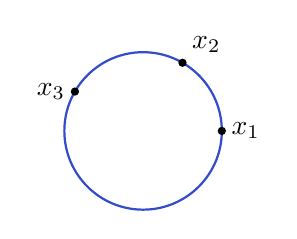
\begin{tikzpicture}
        \draw [mblue, thick] circle [radius=1];
        \node [circ] at (1, 0) {};
        \node [right] at (1, 0) {$x_1$};
        \node [circ] at (0.5, 0.866) {};
        \node [anchor = south west] at (0.5, 0.866) {$x_2$};
        \node [circ] at (-0.866, 0.5) {};
        \node [left] at (-0.866, 0.5) {$x_3$};
      \end{tikzpicture}
    \end{center}
    Formally, we let $\tilde{x} \in \R$ be any lift of $x_1$. Then let $\tilde{x}_2, \tilde{x}_3$ be the unique lifts of $x_2$ and $x_3$ respectively to $[\tilde{x}_1, \tilde{x}_1 + 1)$. Then we say $x_1, x_2, x_3$ are $+$-oriented if $\tilde{x}_2 < \tilde{x}_3$.

      We say $\varphi$ is orientation preserving if it maps any $+$-oriented triple to a $+$-oriented triple.
\end{itemize}

It is an exercise to the following:
\begin{prop}
  Every lift of $\tilde{\varphi}: \R \to \R$ of an orientation preserving $\varphi: S^1 \to S^1$ is a monotone increasing homeomorphism of $\R$, commuting with translation by $\Z$, i.e.
  \[
    \tilde{\varphi} \circ T_m = T_m \circ \tilde{\varphi}
  \]
  for all $m \in \Z$.

  Conversely, any such map is a lift of an orientation-preserving homeomorphism.
\end{prop}

In terms of group theory, the group
\[
  \Homeo^+_\Z(\R) = \left\{\parbox{7cm}{$f: \R \to \R$ monotone increasing homeomorphisms commuting with $T_\Z$}\right\}
\]
is a \term{central extension} of $\Homeo^+(S^1)$ by $\Z$. This means we have an exact sequence of groups
\[
  \begin{tikzcd}[row sep=tiny]
   0 \ar[r] & \Z \ar[r, "i"] & \Homeo_\Z^+ (\R) \ar[r, "p"] & \Homeo^+(S^1) \ar[r] & 0\\
   & m \ar[r, maps to] & T_m
  \end{tikzcd},
\]
where the ``central'' part refers to the fact that the image of $\Z$ is in the center of $\Homeo_\Z^+(\R)$.

Observe that $T_\R \subseteq \Homeo_\Z^+(\R)$ and its image in $\Homeo^+(S^1)$ is the group of rotations, which we denote \term{$\Rot$}.

From a topological point of view, we can see that $\Homeo^+(S^1)$ retracts to $\Rot$. More precisely, if we fix a basepoint $x_0 \in S_1$, and write $\Homeo^+(S^1, x_0)$ for the basepoint preserving maps, then every element in $\Homeo^+(S^1)$ is a product of an element in $\Rot$ and one in $\Homeo^+(S^1, x_0)$. Since $\Homeo^+(S^1, x_0) \cong \Homeo^+([0, 1])$ is contractible, it follows that $\Homeo^+(S^1)$ retracts to $\Rot$. Then a bit more fiddling around with the exact sequence above shows that that is in fact a universal covering space, and that $\pi_1(\Homeo^+(S^1)) = \Z$.

\begin{lemma}
  The map $F: \Homeo_\Z^+(\R) \to \R$ given by $\varphi \mapsto \varphi(0)$ is a quasi-homomorphism.
\end{lemma}

\begin{proof}
  The commutation property of $\varphi$ reads as follows:
  \[
    \varphi(x + m) = \varphi(x) + m.
  \]
  For a real number $x \in \R$, we write
  \[
    x = \{x \} + [x],
  \]
  where $0 \leq \{x\} < 1$ and $[x] = 1$. Then we have
  \begin{align*}
    F(\varphi_1 \varphi_2) &= \varphi_1(\varphi_2(0)) \\
    &= \varphi_1(\varphi_2(0))\\
    &= \varphi_1(\{\varphi_2(0)\} + [\varphi_2(0)])\\
    &= \varphi_1(\{\varphi_2(0)\}) + [\varphi_2(0)]\\
    &= \varphi_1(\{\varphi_2(0)\}) + \varphi_2(0) - \{\varphi_2(0)\}.
  \end{align*}
  Since $0 \leq \{\varphi_2(0)\} < 1$, we know that
  \[
    \varphi_1(0) \leq \varphi_1(\{\varphi_2(0)\}) < \varphi_1(1) = \varphi_1(0) + 1.
  \]
  Then we have
  \[
    \varphi_1(0) + \varphi_2(0) - \{\varphi_2(0)\} \leq F(\varphi_1\varphi_2) < \varphi_1(0) + 1 + \varphi_2(0) - \{\varphi_2(0)\}.
  \]
  So subtracting, we find that
  \[
    -1 \leq - \{\varphi_2(0)\} \leq F(\varphi_1 \varphi_2) - F(\varphi_1) - F(\varphi_2) < 1 - \{\varphi_2(0) \} \leq 1.
  \]
  So we find that
  \[
    D(f) \leq 1.
  \]
\end{proof}

\begin{defi}[Poincare translation quasimorphism]\index{Poincare translation quasimorphism}
  The \emph{Poincare translation quasimorphism} $T: \Homeo_\Z^+ (\R) \to \R$ is the homogenization of $F$.
\end{defi}

It is easily seen that $T(T_x) = x$. This allows us to define

\begin{defi}[Rotation number]\index{rotation number}
  The \emph{rotation number} \index{$R(\varphi)$} of $\varphi \in \Homeo^+(S^1)$ is $T(\tilde{\varphi}) \bmod \Z \in \R/\Z$.
\end{defi}
This rotation number contains a lot of interesting information about the dynamics of the homeomorphism. For instance, minimal homeomorphisms of $S^1$ are conjugate iff they have the same rotation number (a minimal homeomorphism is one such that every orbit is dense).

We will see that bounded cohomology allows us to generalize the rotation number of a homeomorphism into an invariant for any group action.

\section{Group cohomology and bounded cohomology}
\subsection{Group cohomology}
Let $A$ be an abelian group, which will later be set to $\Z$ or $\R$. To a group $\Gamma$, we are going to associate a sequence of abelian groups $H^k(\Gamma, A)$ that is
\begin{itemize}
  \item covariant in $A$; and
  \item contravariant in $\Gamma$.
\end{itemize}
Moreover, if $\Gamma = \pi_1(X)$, where $X$ is an aspherical CW-complex (i.e.\ one with contractible universal cover), then we have a natural isomorphism
\[
  H^k(\Gamma, A) \cong H^k_{\mathrm{sing}}(X, A).
\]

To do so, we need to make some definitions.
\begin{defi}[Homogeneous $k$-cochain]\index{$k$-cochain}\index{homogeneous $k$-cochain}\index{cochain}
  A \emph{homogeneous $k$-cochain} with values in $A$ is a map $f: \Gamma^{k + 1} \to A$. The set \term{$C(\Gamma^{k + 1}, A)$} is an abelian group and $\Gamma$ acts on it by automorphisms in the following way:
  \[
    (\gamma_* f) (\gamma_0, \cdots, \gamma_m) = f(\gamma^{-1} \gamma_0, \cdots, \gamma^{-1} \gamma_k).
  \]
  By convention, we set $C(\Gamma^0, A) \cong A$.
\end{defi}

We organize this into a \emph{complex} of abelian groups
\[
  \begin{tikzcd}
    0 \ar[r] & A \ar[r, "d^{(0)}"] & C(\Gamma, A) \ar[r, "d^{(1)}"] & \cdots
  \end{tikzcd}
\]
where for $f \in C(\Gamma^k, A)$, we set
\[
  (d^{(k)}f) (\gamma_0, \cdots, \gamma_k) = \sum_{j = 0}^k (-1)^j f(\gamma_0, \cdots, \hat{\gamma}_j, \cdots, \gamma_k).
\]
In particular, we set $d^{(0)}(a)$ to be the constant $a$ function.

\begin{eg}
  We have
  \begin{align*}
    d^{(1)} f(\gamma_0, \gamma_1) &= f(\gamma_1) - f(\gamma_0)\\
    d^{(2)} f(\gamma_0, \gamma_1, \gamma_2) &= f(\gamma_1, \gamma_2) - f(\gamma_0, \gamma_2) + f(\gamma_0, \gamma_1).
  \end{align*}
\end{eg}

\begin{defi}[$k$-cocycle and $k$-coboundaries]\index{$k$-cocycle}\index{$k$-coboundary}\index{cocycle}\index{coboundary}
  The $k$-cocycles are $\ker d^{(k + 1)}$.
  The $k$-coboundaries are $\im d^{(k)}$.
\end{defi}

\begin{lemma}\leavevmode
  \begin{enumerate}
    \item $d^{(k)}$ is a $\Gamma$-equivariant group homomorphism.
    \item $d^{(k + 1)} \circ d^{(k)} = 0 $. So $\im d^{(k)} \subseteq \ker d^{(k + 1)}$.
    \item In fact, we have $\im d^{(k)} = \ker d^{(k + 1)}$.
  \end{enumerate}
\end{lemma}

\begin{proof}\leavevmode
  \begin{enumerate}
    \item This is clear.
    \item You just expand it out and see it is zero.
    \item If $f \in \ker d^{(k)}$, then setting $\gamma_k = e$, we have
      \begin{multline*}
        d^{(k)} f(\gamma_0, \cdots, \gamma_{k - 1}, e) = (-1)^k f(\gamma_0, \cdots, \gamma_{k - 1}) \\
        + \sum_{j = 0}^{k - 1} (-1)^j f(\gamma_0, \cdots, \hat{\gamma}_j, \cdots, \gamma_{k - 1}, e) = 0.
      \end{multline*}
      Now define the following $k - 1$-cochain
      \[
        h(\gamma_0, \cdots, \gamma_{k - 2}) = (-1)^k f(\gamma_0, \cdots, \gamma_{k - 2}, e).
      \]
      Then the above reads
      \[
        f = d^{(k - 1)} h.
      \]
  \end{enumerate}
\end{proof}
Recall that there is an action of $\Gamma$ on $C(\Gamma^k, A)$. We now let
\[
  C(\Gamma^k, A)^\Gamma = \{f: \Gamma^k \to A \mid f \text{ is $\Gamma$-invariant}\}.
\]
Since the differentials $d^{(k)}$ commute with the $\Gamma$-action, it restricts to a map $d^{(k)}|_{C(\Gamma^k, A)^\Gamma} : C(\Gamma^k, A)^\Gamma \to C(\Gamma^{k + 1}, A)^\Gamma$.

In particular, we have $d^{(k)} (C(\Gamma^k, A)^\Gamma) \subseteq (\ker d^{(k + 1)})^\Gamma$.

We are now in a position to define group cohomology.
\begin{defi}[Group cohomology $H^k(\Gamma, A)$]\index{$H^k(\Gamma, A)$}\index{group cohomology}
  We define the \emph{$k$th cohomology group} to be
  \[
    H^k = \frac{(\ker d^{(k + 1)})^\Gamma}{d^{(k)} (C(\Gamma^k, A)^\Gamma)} = \frac{(d^{(k)} (C(\Gamma^k, A)))^\Gamma}{d^{(k)} (C(\Gamma^k, A)^\Gamma)}.
  \]
\end{defi}

We can alternatively provide a model with \term{inhomogeneous cochains}. It is simply the following observation --- if we have a function $f: \Gamma^{k + 1} \to A$ that is invariant under the action of $\Gamma$, then it is uniquely determined by the value of $\{(e, \gamma_1, \cdots, \gamma_k): \gamma_i \in \Gamma\}$. So we can identify invariant functions $f: \Gamma^{k + 1} \to A$ with arbitrary functions $\Gamma^k \to A$. So we have one variable less to worry about, but on the other hand, the coboundary maps are much more complicated.

More explicitly, we construct an isomorphism
\[
  \begin{tikzcd}
    C(\Gamma^k, A)^\Gamma \ar[r, yshift=2, "\rho^{(k - 1)}"] & C(\Gamma^{k - 1}, A)\ar[l, yshift=-2, "\tau^{(k)}"]
  \end{tikzcd},
\]
by setting
\begin{align*}
  (\rho^{(k - 1)} f)(g_1, \cdots, g_{k - 1}) &= f(e, g_1, g_2, \cdots, g_1 \cdots g_{k - 1})\\
  (\tau^{(k)} h)(g_1, \cdots, g_k) &= h (g_1^{-1} g_2, g_2^{-1} g_3, \cdots, g_{k - 1}^{-1} g_k).
\end{align*}

These homomorphisms are inverses of each other. Then under this identification, we obtain a new complex
\[
  \begin{tikzcd}
    C(\Gamma^k, A)^\Gamma \ar[r, "d^{(k)}"] & C(\Gamma^{k + 1}, A)^\Gamma \ar[d,"\rho^{(k)}"] \\
    C(\Gamma^{k - 1}, A) \ar[u, "\tau^{(k)}"]  \ar[r,  "d^{k}"] & C(\Gamma^k, A)
  \end{tikzcd}
\]
where
\[
  d^k = \rho^k d^{(k)} \tau^k.
\]
A computation shows that
\begin{align*}
  (d^k f) (g_1, \cdots, g_k) = f(g_2, \cdots, g_k) + \sum_{j = 1}^{k - 1} (-1)^j f(g_1, \cdots, g_j g_{j + 1},  \cdots, g_k) \\
  + (-1)^k f(g_1, \cdots, g_{k - 1}).
\end{align*}
It is customary to denote
\begin{align*}
  \mathcal{Z}^k(\Gamma, A) &= \ker^{d + 1} \subseteq C(\Gamma^k, A)\\
  \mathcal{B}^k (\Gamma, A) &= \im d^k \subseteq C(\Gamma^k, A),
\end{align*}
the \term{inhomogeneous $k$-cocycles}\index{$k$-cocycle!inhomogeneous}\index{cocycle!inhomogeneous} and \term{inhomogeneous $k$-coboundaries}\index{$k$-coboundary!inhomogeneous}\index{coboundary!inhomogeneous}.

\subsubsection*{Computation in degree $k = 0, 1, 2$}
\begin{itemize}
  \item For $H^0(\Gamma, A)$, the relevant part of the cochain is
    \[
      \begin{tikzcd}
        0 \ar[r] & A \ar[r, "d^1 = 0"] & C(\Gamma, A)
      \end{tikzcd}.
    \]
    So we see that $H^0(\Gamma, A) \cong A$.

  \item For $H^1(\Gamma, A)$, the relevant part is
    \[
      \begin{tikzcd}
        A \ar[r, "d^1 = 0"] & C(\Gamma, A) \ar[r, "d^2"] & C(\Gamma^2, A)
      \end{tikzcd}.
    \]
    Then we have
    \[
      (d^2 f) (\gamma_1, \gamma_2) = f(\gamma_1 - f(\gamma_1 \gamma_2) + f(\gamma_2).
    \]
    So we find that $H^1(\Gamma, A) = \Hom(\Gamma, A)$.
  \item For $H^2(\Gamma, A)$, the relevant part is
    \[
      \begin{tikzcd}
        C(\Gamma, A) \ar[r, "d^2"] & C(\Gamma^2, A) \ar[r, "d^3"] & C(\Gamma^3, A)
      \end{tikzcd}.
    \]
    Here $d^3$ is given by
    \[
      d^3 \alpha (g_1, g_2, g_3) = \alpha(g_2, g_3) - \alpha(g_1 g_2, g_3) + \alpha(g_1, g_2 g_3) - \alpha(g_1, g_2).
    \]
\end{itemize}
What can this $H^3(\Gamma, A)$ possibly mean? It is not so obvious this time, but it still has a nice interpretation.

Suppose that $d^3 \alpha (g_1, g_2, g_3) = 0$. In addition, by some magic, we managed to pick $\alpha$ such that $\alpha(g_1, e) = \alpha(e, g_2) = 0$. This is known as a \term{normalized cocycle}. We can now define the following operation on $\Gamma \times A$:
\[
  (\gamma_1, a_2)(\gamma_2, a_2) = (\gamma_1 \gamma_2, a_1 +a _2 + \alpha (\gamma_1, \gamma_2)).
\]
Then the property that $\alpha$ is a normalized cocycle is equivalent to the assertion that this is an associative group law with identity elements $(e, 0)$. We will write this group as $\Gamma \times_\alpha A$.

We can think of this as a generalized version of the semi-direct product. This group here has a special property. We can organize it into an exact sequence
\[
  \begin{tikzcd}
    0 \ar[r] & A \ar[r] & \Gamma \times_\alpha A \ar[r] & \Gamma \ar[r] & 0
  \end{tikzcd}.
\]
Moreover, the image of $A$ is in the center of $\Gamma \times_\alpha A$. This is known as a \term{central extension}.
\begin{defi}[Central extension]\index{central extension}
  Let $A$ be an abelian group, and $\Gamma$ a group. Then a central extension of $\Gamma$ by $A$ is an exact sequence
  \[
    \begin{tikzcd}
      0 \ar[r] & A \ar[r] & \tilde{\Gamma} \ar[r] & \Gamma \ar[r] & 0
    \end{tikzcd}
  \]
  such that the image of $A$ is contained in the center of $\tilde{\Gamma}$.
\end{defi}
The claim is now that

\begin{prop}
  $H^2(\Gamma, A)$ parametrizes the set of isomorphism classes of central extensions of $\Gamma$ by $A$.
\end{prop}

\begin{proof}[Proof sketch]
  Consider a central extension
  \[
    \begin{tikzcd}
      0 \ar[r] & A \ar[r, "i"] & G \ar[r, "p"] & \Gamma \ar[r] & 0
    \end{tikzcd}.
  \]
  Arbitrarily choose a section $s: \Gamma \to G$ of $p$, as a function of sets. Then we know there is a unique $\alpha(\gamma_1, \gamma_2)$ such that
  \[
    s(\gamma_1 \gamma_2) \alpha(\gamma_1, \gamma_2) = s(\gamma_1) s(\gamma_2).
  \]
  We then check that $\alpha$ is a (normalized) $2$-cocycle, i.e.\ $\alpha(\gamma_1, e) = \gamma(e, \gamma_2) = 0$.

  One then verifies that different choices of $s$ gives cohomologous choices of $\alpha$.

  Conversely, given a $2$-cocycle $\beta$, we can show that it is cohomologous to a normalized $2$-cocycle $\alpha$. This gives rise to a central extension $G = \Gamma \times_\alpha A$ as constructed before (and also a canonical section $s(\gamma) = (\gamma, 0)$).

  One then checks this is a bijection.
\end{proof}

\begin{ex}
  $H^2(\Gamma, A)$ has a natural structure as an abelian group. Then by the proposition, we should be able to ``add'' two central extensions.
\end{ex}

\begin{eg}
  As usual, write $\F_r$ for the free group on $r$ generators. Then
  \begin{align*}
    H^k(\F_r, A) = 
    \begin{cases}
      A & k = 0\\
      A^r & k = 1\\
      0 & k = 2
    \end{cases}.
  \end{align*}
  The fact that $H^2(\F_r, A)$ vanishes is due to the fact that $\F_r$ is free, so every short exact sequence splits.
\end{eg}

\begin{eg}
  If $\Gamma_g$ is the fundamental group of the orientable surface of genus $g$, then
  \[
    H^2 (\Gamma_g, \Z) \cong \Z.
  \]
\end{eg}

\begin{eg}
  The central extension
  \[
    \begin{tikzcd}
      0 \ar[r] & \Z \ar[r, "i"] & \Homeo^+_\Z(\R) \ar[r, "p"] & \Homeo^+(S^1) \ar[r] & 0
    \end{tikzcd}
  \]
  gives rise to the \term{Euler class} $e \in H^2(\Homeo^+(S^1), \Z)$.

  Let's construct a representative cocycle. To do so, we pick a section $s: \Homeo^+(S^1) \to \Homeo_\Z^+(\R)$ by sending $f \in \Homeo^+(S^1)$ to the unique lift $\bar{f}: \R \to \R$ such that $\bar{f}(0) \in [0, 1)$.

  Then we find that
  \[
    s(f_1, f_2) T_{c(f_1, f_2)} = s(f_1) s(f_2)
  \]
  for some $c(f_1, f_2) \in \Z$.
\end{eg}

\begin{lemma}
  We have $c(F_1, f_2) \in \{0, 1\}$.
\end{lemma}

\begin{proof}
  We have $\overline{f_1 f_2}(0) \in [0, 1)$, while $\bar{f}_2(0) \in [0, 1)$. So we find that
  \[
    \bar{f}_1(\bar{f}_2(0)) \in [\bar{f}_1(0), \bar{f}_1(1)) = [\bar{f}_1(0), \bar{f}_1(0) + 1) \subseteq [0, 2).
  \]
  But we also know that $c(f_1, f_2)$ is an integer. So $c(f_1, f_2) \in \{0, 1\}$.
\end{proof}

\begin{eg}
  Consider $\Gamma_g = \pi_1(S_g)$ for $g \geq 0$. Explicitly, we can write
  \[
    \Gamma_g = \left\{a_1, b_1, \cdots, a_g, b_g : \prod_{i = 1}^g [a_i, b_i] = e\right\}
  \]
  Then we have $H^1(\Gamma_g, \Z) = \Z^{2g}$ and $H^2(\Gamma_g, \Z) \cong \Z$.

  We can provide a very explicit isomorphism for $H^2(\Gamma_g, \Z)$. We let
  \[
    \begin{tikzcd}
      0 \ar[r] & \Z \ar[r, "i"] & G \ar[r, "p"] & \Gamma \ar[r] & 0
    \end{tikzcd}
  \]
  be a central extension. Observe that whenever $\gamma, \eta \in \Gamma_g$, and lets $\tilde{\gamma}, \tilde{\eta} \in G$, then $[\tilde{\gamma}, \tilde{\eta}]$ is a lift of $[\gamma, \eta]$, and doesn't depend on the choice of the lifts. Now pick $\tilde{a}_1, \tilde{b}_1, \cdots, \tilde{a}_g, \tilde{b}_g$. Then notice that
  \[
    \prod_{i = 1}^g [\tilde{a}_i, \tilde{b}_i] \in \Z
  \]
  is in the kernel of $p$, and is hence in $\Z$.
\end{eg}

\begin{defi}[Euler class]\index{Euler class}
  The \emph{Euler class} of the $\Gamma$-action by orientation-preserving homeomorphisms of $S^1$ is
  \[
    h^*(e) \in H^2(\Gamma, \Z),
  \]
  where $h: \Gamma \to \Homeo^+(S^1)$ is the map defining the action.
\end{defi}

For example, if $\Gamma_g$ is a surface group, then we obtain an invariant of actions valued in $\Z$.  

There are some interesting theorems about this Euler class that we will not prove.
\begin{thm}[Milnor--Wood]
  We have $|h^*(e)| \leq 2g - 2$.
\end{thm}

\begin{thm}[Gauss--Bonnet]
  If $h: \Gamma_g \to \PSL(2, \R) \subseteq \Homeo^+(S^1)$ is the holonomy representation of a hyperbolic structure, then
  \[
    h^*(e) = \pm (2g - 2).
  \]
\end{thm}

\begin{thm}[Matsumoko, 1986]
  If $h$ defines a miimal action of $\Gamma_g$ on $S^1$ and $|h^*(e)| = 2g - 2$, then $h$ is conjugate to a hyperbolization.
\end{thm}

\subsection{Bounded cohomology of groups}
We now take $A = \Z$ or $\R$, since they are the groups we know what ``bounded'' means.

We let\index{$C_b(\Gamma^{k + 1}, A)$}
\[
  C_b(\Gamma^{k + 1}, A) = \{f \in C(\Gamma^{k + 1}, A) : f\text{ is bounded}\} \subseteq C(\Gamma^{k + 1}, A).
\]
We have that $d^{(k)}(C_b(\Gamma^k, A)) \subseteq C_b(\Gamma^{k + 1}, A)$, and hence we have
\[
  d^{(k)}(C_b(\Gamma^k, A)^\Gamma) \subseteq C_b(\Gamma^{k + 1}, A)^\Gamma.
\]
This allows us to define

\begin{defi}[Bounded cohomology]\index{bounded cohomology}\index{$k$-th bounded cohomology}
  The \emph{$k$-th bounded cohomology group} of $\Gamma$ with coefficients in $A$ Is
  \[
    H_b^k(\Gamma, A) = \frac{\ker (d^{(k + 1)} : C_b(\Gamma^{k + 1}, A)^\Gamma \to C_b(\Gamma^{k + 2}, A)^\Gamma)}{d^{(k)}(C_b(\Gamma^k, A)^\Gamma)}.
  \]
\end{defi}

This comes with two additional features.
\begin{enumerate}
  \item A bounded cochain is bounded. So for $f \in C_b(\Gamma^{k + 1}, A)$, we define
    \[
      \|f\|_\infty = \sup_{x \in \Gamma^{k + 1}} |f(x)|.
    \]
    Then $\|\ph\|_\infty$ makes $C-b(\Gamma^{k + 1}, A)$ into a normed abelian group, and in the case $A = \R$, a Banach space.

    Then for $[f] \in H^k_b(\Gamma, A)$, we define
    \[
      \|[f]\|_\infty = \inf \{ \|f + d g\|_\infty : g \in C_b(\Gamma^k, A)^\Gamma\}.
    \]
    This induces a semi-norm on $H^k_b(\Gamma, A)$. This is called the \term{canonical semi-norm}.
  \item We have a map of chain complexes
    \[
      \begin{tikzcd}
        C_b(\Gamma, A)^\Gamma \ar[r] \ar[d,  hook] & C_b(\Gamma^2, A)^\Gamma \ar[r] \ar[d, hook] & C_b(\Gamma^3, A)^\Gamma \ar[r] \ar[d, hook] & \cdots\\
        C(\Gamma, A)^\Gamma \ar[r] & C(\Gamma^2, A)^\Gamma \ar[r] & C(\Gamma^3, A)^\Gamma \ar[r] & \cdots
      \end{tikzcd}
    \]
    Thus, this induces a natural map $c_k: H^k_b (\Gamma, A) \to H^k(\Gamma, A)$, known as the \term{comparison map}. In general, $c_k$ need not be injective or surjective.
\end{enumerate}

As before, we can instead use the complex of inhomogeneous cochains. Then we have a complex that looks like
\[
  \begin{tikzcd}
    0 \ar[r] & A \ar[r, "d^1 = 0"] & C_b(\Gamma, A) \ar[r,  "d^2"] & C_b(\Gamma^2, A) \ar[r, "d^3"] & \cdots
  \end{tikzcd}
\]
In degree $0$, the boundedness condition is useless, and we have
\[
  H_b^0(\Gamma, A) = H^0(\Gamma, A) = A.
\]
For $k = 1$, we have $\im d^1 = 0$. So we just have to compute the cocycles. For $f \in C_b(\Gamma, A)$, we have $d^2 f = 0$ iff $f(g_1) - f(g_1 g_2) + f(g_2) = 0$, iff $f \in \Hom(\Gamma, A)$. But we have the additional information that $f$ is bounded. But there are no non-zero bounded homomorphisms to $\Gamma$ or $A$! So we have
\[
  H_b^1(\Gamma, A) = 0.
\]
Later, when we allow non-trivial coefficients, then $H^1_b(\Gamma, A)$ will not always be zero.

We now look at $H_b^2(\Gamma, A)$. We are going to determine the kernel of the comparison map
\[
  c_2; H_b^2(\Gamma, A) \to H^2(\Gamma, A).
\]
We consider the relevant of the defining complexes, where we take inhomogeneous cochains
\[
  \begin{tikzcd}
    C(\Gamma, A) \ar[r, "d^2"] & C(\Gamma^2, A) \ar[r, "d^3"] & C(\Gamma^3, A)\\
    C_b(\Gamma, A) \ar[r, "d^2"] \ar[u, hook] & C_b(\Gamma^2, A) \ar[r, "d^3"] \ar[u, hook] & C_b(\Gamma^3, A) \ar[u, hook]
  \end{tikzcd}
\]
Then the kernel of $c_2$ consists of the $[\alpha] \in H^2_b(\Gamma, A)$ such that $\alpha = d^2 f$ for some $f \in C(\Gamma, A)$. But $d^2 f = \alpha$ being bounded tells us $f$ is a quasi-homomorphism! Thus, we have a map
\[
  \begin{tikzcd}[cdmap]
    \bar{d}^2: \QH(\Gamma, A) \ar[r] & \ker c_2\\
    f \ar[r, maps to] *& [ d^2 f].
  \end{tikzcd}
\]
\begin{prop}
  The map $\bar{d}^2$ induces an isomorphism
  \[
    \frac{\QH(\Gamma, A)}{\ell^\infty(\Gamma, A) + \Hom(\Gamma, A)} \cong \ker c_2.
  \]
\end{prop}

\begin{proof}
  We know that $\bar{d}^2$ is surjective. So it suffices to show that the kernel is $\ell^\infty(\Gamma, A) + \Hom(\Gamma, A)$.

  Suppose $f \in \QH(\Gamma, A)$ is such that $\bar{d}^2 f \in H_b^2(\Gamma, A) = 0$. Then there exists some $g \in C_b(\Gamma, A)$ such that
  \[
    d^2 f = d^g.
  \]
  So ti follows that $d^2 (f - g) = 0$. That is, $f - g \in \Hom(\Gamma, A)$. Hence it follows that
  \[
    \ker \bar{d}^2 \subseteq \ell^\infty(\Gamma, A) + \Hom(\Gamma, A).
  \]
  The other inclusion is clear.
\end{proof}

\begin{eg}\leavevmode
  \begin{itemize}
    \item For $G$ abelian and $A = \R$, we saw that $\QH(\Gamma, A) = \ell^\infty(\Gamma, A) + \Hom(\Gamma, A)$. So it follows that $c_2$ is injective.
    \item For $H^2_b(\Z, \Z)$, we know $H^2(\Z, \Z) = 0$ since $\Z$ is a free group (hence, e.g.\ every extension splits, and in particular all central extensions do). Then we know
      \[
        H_b^2 (\Z, \Z) \cong \frac{\QH(\Z, \Z)}{\ell^\infty(\Z, \Z) + \Hom(\Z, \Z)} \cong \R / \Z.
      \]
      To see this isomorphism, for any $\alpha \in \R$, we define
      \[
        g_\alpha(m) = [m \alpha].
      \]
      Then $g_\alpha \in \QH(\Z, \Z)$. Then the map
      \[
        \R \to \frac{\QH(\Z, \Z)}{\ell^\infty(\Z, \Z)},
      \]
      is a group isomorphism. This induces an isomorphism
      \[
        \R/\Q \cong \frac{\QH(\Z, \Z)}{\ell^\infty(\Z, \Z) + \Hom(\Z, \Z)} \cong H_b^2(\Z, \Z).
      \]
    \item Consider $H_b^2(\F_r, \Q)$. We know that $H^2 (\F_r, \R) = 0$. By Rollis' theorem, we have an inclusion
      \[
        \begin{tikzcd}[cdmap]
          \ell^\infty_{\mathrm{odd}}(\Z, \R) \oplus \ell^\infty_{\mathrm{odd}}(\Z, \R) \ar[r] & H^2_b(\F_r, \R)\\
          (\alpha, \beta) \ar[r, maps to] & \lbrack d^2 f_{\alpha, \beta}\rbrack
        \end{tikzcd}
      \]
      Recall that $H_b^2(\F_r, \R)$ has the structure of a semi-normed space, which we called the canonical norm. One can show that
      \[
        \|[d^2 f_{\alpha, \beta}]\| = \max (\|d \alpha\|_\infty, \|d \beta\|_\infty).
      \]
    \item We have a Gersten long exact sequence (1992) as follows: % check spelling, 1992

      Consider the exact sequence of abelian groups
      \[
        \begin{tikzcd}
          0 \ar[r] & \Z \ar[r] & \R \ar[r] & \R/\Z \ar[r] & 0
        \end{tikzcd}.
      \]
      By homological algebra, we obtain a short exact sequence of chain complexes
      \[
        \begin{tikzcd}
          0 \ar[r] & C_b (\Gamma^\Cdot, \Z) \ar[r] & C_b (\Gamma^\Cdot, \R) \ar[r] & C(\Gamma^\Cdot, \R/\Z) \ar[r] & 0
        \end{tikzcd}
      \]
      One should check carefully that this is indeed correct, and in particular we don't have a subscript $b$ in the $\R/\Z$ complex. Then by the snake lemma, we obtain a long exact sequence
      \[
        \begin{tikzcd}
           H^{k - 1}(\Gamma, \R/\Z) \ar[r, "\delta"] & H^k_b(\Gamma, \Z) \ar[r] & H_b^k(\Gamma, \R) \ar[r] & H^k(\Gamma, \R/\Z)
        \end{tikzcd}.
      \]
      So for example, we have
      \[
        \begin{tikzcd}
          0 = H_b^1(\Gamma, \R) \ar[r] & \Hom(\Gamma, \R/Z) \ar[r, "\delta"] & H_b^2(\Gamma, \Z) \ar[r] & H_b^2(\Gamma, \R)
        \end{tikzcd}.
      \]
      So in the case $\Gamma = \Z$, since $\Gamma$ is abelian, we recover the isomorphism
      \[
        \R/\Z = \Hom(\Z, \R/\Z) \cong H_b^2(\Z, \Z).
      \]
    \item In Gersten's \emph{Bounded cocycles and combing of groups} (1992) paper, it is shown that the image of the comparison map $c_2; H_b^2(\Gamma, \Z) \to H^2(\Gamma, \Z)$ describes central extensions with special metric features.

      \begin{thm}
        Assume $\Gamma$ is finitely-generated. Let $G_\alpha$ be the central extension of $\Gamma$ by $\Z$, defined by a class in $H^2(\Gamma, \Z)$ which admits a bounded representative. Then with any word metric, $\Gamma_\alpha$ is quasi-isometric to $\Gamma \times \Z$ via the ``identity map''.
      \end{thm}

      A typical application is as follows --- for $n \geq 2$, the preimage $\tilde{\Gamma}$ of $\Sp(2n, \Z)$ in the universal covering of $\Sp(2n, \R)$ is a central $\Z$-extension of the above type. In addition, $\tilde{\Gamma}$ has property (T). But $\Gamma \times \Z$ doesn't have property (T). 
  \end{itemize}
\end{eg}

One of the most important features of bounded cohomology is that (for real coefficients) it vanishes for amenable groups.
\begin{defi}[Amenable group]\index{amenable group}
  A discrete group $\Gamma$ is \emph{amenable} if there is a linear form $m: \ell^\infty(\Gamma,\R) \to \R$ such that
  \begin{itemize}
    \item $m(f) \geq 0$ if $f \geq 0$;
    \item $m(1) = 1$; and
    \item $m$ is left-invariant, i.e.\ $m(\gamma_* f) = m(f)$, where $(\gamma_* f)(x) = f(\gamma^{-1}x)$.
  \end{itemize}
\end{defi}
A linear form that satisfies the first two properties is known as a \term{mean}, and we can think of this as a way of integrating functions. Then an amenable group is a group with a left invariant mean. Note that the first two properties imply
\[
  |m(f)| \leq \|f\|_\infty.
\]
\begin{eg}\leavevmode
  \begin{itemize}
    \item Abelian groups are amenable, and finite groups are.
    \item Subgroups of amenable groups are amenable.
    \item If
      \[
        \begin{tikzcd}
          0 \ar[r] & \Gamma_1 \ar[r] & \Gamma_2 \ar[r] & \Gamma_3 \ar[r] & 0
        \end{tikzcd}
      \]
      is a short exact sequence, then $\Gamma_2$ is amenable iff $\Gamma_1$ and $\Gamma_3$ are amenable.
    \item Let $\Gamma = \bra S \ket$ for $S$ a finite set. Given a finite set $A \subseteq \Gamma$, we define $\partial A$ to be the set of all edges with exactly one vertex in $A$.

      For example, $\Z^2$ with the canonical generators has Cayley graph
      \begin{center}
        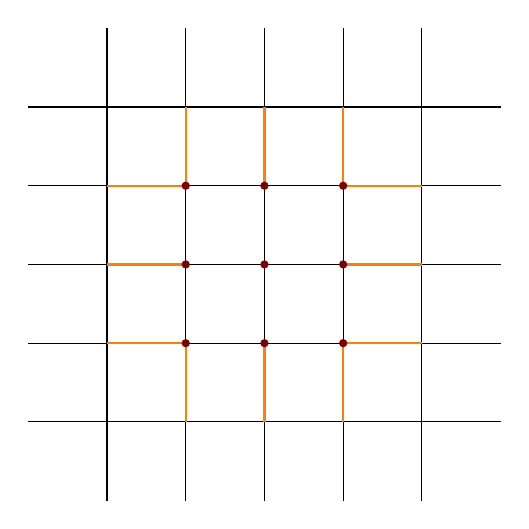
\begin{tikzpicture}
          \foreach \x in {-2, -1, 0, 1, 2} {
             \draw (\x, -3) -- (\x, 3);
             \draw (-3, \x) -- (3, \x);
          }
          \foreach \x in {-1, 0, 1} {
            \draw [morange, thick] (1, \x) -- (2, \x);
            \draw [morange, thick] (-1, \x) -- (-2, \x);
            \draw [morange, thick] (\x, 1) -- (\x, 2);
            \draw [morange, thick] (\x, -1) -- (\x, -2);
          }
          \foreach \x in {-1, 0, 1} {
             \foreach \y in {-1, 0, 1} {
               \node [circ, mred] at (\x,  \y) {};
            }
          }
        \end{tikzpicture}
      \end{center}
      Then if $A$ consists of the red points, then the boundary consists of the orange edges.

      Then $\Gamma$ is non-amenable iff there exists $c (s, \Gamma) > 0$ such that for all $A \subseteq \Gamma$, we have $|\partial A| \geq c|A|$.
    \item There exists infinite, finitely generated, simple, anemable groups.
    \item If $\Gamma \subseteq \GL(n, \C)$, then $\Gamma$ is amenable iff it contains a finite-index subgroup which is solvable.
    \item $\F_2$ is non-amenable.
    \item Any non-elementary word-hyperbolic group is non-amenable.
  \end{itemize}
\end{eg}

So quite a few groups are non-amenable. Which is good, because now the following vanishing theorem would not apply!

\begin{prop}
  Let $\Gamma$ be an amenable group. Then $H^k_b(\Gamma, \R) = 0$ for $k \geq 1$.
\end{prop}

The proof requires absolutely no idea.
\begin{proof}
  Let $k \geq 1$ and $f: \Gamma^{k + 1} \to \R$ a $\Gamma$-invariant bounded cocycle. In other words,
  \begin{align*}
    d^{(k + 1)} f &= 0\\
    f(\gamma\gamma_0, \cdots, \gamma\gamma_k) &= f(\gamma_0, \cdots, \gamma_k).
  \end{align*}
  We have to find $\varphi: \Gamma^k \to \R$ bounded such that
  \begin{align*}
    d^{(k)} \varphi &= f\\
    \varphi(\gamma\gamma_0, \cdots, \gamma_{k - 1}) &= \varphi(\gamma_0, \cdots, \gamma_{k - 1}).
  \end{align*}
  Recall that for $\eta \in \Gamma$, we can define
  \[
    h_\eta (\gamma_0, \cdots, \gamma_{k - 1}) = (-1)^{k + 1} f(\gamma_0, \cdots, \gamma_{k + 1}, \eta),
  \]
  and then
  \[
    d^{(k + 1)}f = 0 \Longleftrightarrow f = d^{(k)}(h_\eta).
  \]
  However, $h_\eta$ need not be invariant. Instead, we have
  \[
    h_\eta(\gamma\gamma_0, \cdots, \gamma\gamma_{k - 1}) = h_{\gamma^{-1} \eta} (\gamma_0, \cdots, \gamma_{k - 1}).
  \]
  Now let $m : \ell^\infty(\Gamma) \to \R$ be a left-invariant mean. We notice that the map
  \[
    \eta \mapsto h_\eta (\gamma_0, \cdots, \gamma_{k - 1})
  \]
  is bounded by $\|f\|_\infty$. So we can define
  \[
    \varphi(\gamma_0, \cdots, \gamma_{k - 1}) = m \Big\{ \eta \mapsto h_\eta (\gamma_0, \cdots, \gamma_{k - 1})\Big\}.
  \]
  Then this is the $\varphi$ we want. Indeed, we have
  \[
    \varphi(\gamma \gamma_0, \cdots, \gamma \gamma_{k - 1}) = m \Big\{ \eta \mapsto h_{\gamma^{-1}\eta} (\gamma_0, \cdots, \gamma_{k - 1})\Big\}.
  \]
  But this is just the mean of a left translation of the original function. So this is just $\varphi(\gamma_0, \cdots, \gamma_{k - 1}$. Also, by properties of the mean, we know $\|\varphi\|_\infty \leq \|f\|_\infty$.

  Finally, by linearity, we have
  \begin{align*}
    d^{(k)} \varphi(\gamma_0, \cdots, \gamma_k) &= m \Big\{ \eta \mapsto d^{(k)} h_\eta (\gamma_0, \cdots, \gamma_k) \Big\}\\
    &= m \Big\{ f(\gamma_0, \cdots, \gamma_k) \cdot \mathbf{1}_\Gamma\Big\}\\
    &= f(\gamma_0, \cdots, \gamma_k) m (\mathbf{1}_\Gamma)\\
    &= f(\gamma_0, \cdots, \gamma_k).
  \end{align*}
\end{proof}

Remember that the central extension
\[
  \begin{tikzcd}
    0 \ar[r] & \Z \ar[r] & \Homeo^+_\Z(\R) \ar[r] & \Homeo^+(S^1) \ar[r] & 0
  \end{tikzcd}
\]
defines the Euler class $e \in H^2(\Homeo^+(S^1), \Z)$. We have also shown that there is a representative cocycle $c(f, g)$ taking the values $\{0, 1\}$, defined by
\[
  \overline{f \circ g} \circ T_{c(f, g)} = \bar{f} \circ \bar{g},
\]
where for any $f$, the map $\bar{f}$ is the unique lift to $\R$ such that $\bar{f}(0) = [0, 1)$.

But in particular, this class is a bounded cocycle. So we can use it to define
\begin{defi}[Bounded Euler class]\index{bounded Euler class}\index{Euler class!bounded}\index{$e^b$}
  The \emph{bounded Euler class}
  \[
    e^b \in H_b^2(\Homeo^+(S^1), \Z)
  \]
  is the bounded cohomology class represented by the cocycle $c$.
\end{defi}

By construction, $e^b$ is sent to $e$ via the comparison map
\[
  \begin{tikzcd}
    c_2: H_b^2(\Homeo^+(S^1), \Z) \ar[r] & H^2(\Homeo^+(S^1), \Z)
  \end{tikzcd}.
\]
In fact, the comparison map is injective. So this $e^b$ is the unique element that is sent to $e$, and doesn't depend on us arbitrarily choosing $c$ as the representative.

\begin{defi}[Bounded Euler class of action]\index{bounded Euler class}\index{Euler class!bounded}
  The bounded Euler class of an action $h: \Gamma \to \Homeo^+(S^1)$ is $h^*(b) \in H_b^2(\Gamma, \Z)$.
\end{defi}

By naturality (proof as exercise), $h^*(e^b)$ maps to $h^*(e)$ under the comparison map. The following is also an exercise:

\begin{ex}
  Show that if $h: \Z \to \Homeo^+(S^1)$ and $\varphi = h(1)$, then under the isomorphism
  \[
    H^2_b(\Z, \Z) \to \R/\Z,
  \]
  we have $h^*(e^b) = \Rot(\varphi)$, the Poincar\'e rotation number of $\varphi$.
\end{ex} % prove this

So this tells us the bounded Euler class is a natural generalization of the Poincar\'e rotation number.

\begin{ex}
  Assume $h: \Gamma \to \Homeo^+(S^1)$  takes values in the rotations $\Rot$. Let $\chi: \Gamma \to \R/\Z$ the corresponding homomorphism. Then under the connecting homomorphism
  \[
    \begin{tikzcd}
      \Hom(\Gamma, \R/\Z) \ar[r, "\delta"] & H_b^2(\Gamma, \Z)
    \end{tikzcd},
  \]
  we have $\delta(\chi) = h^*(e^b)$.
\end{ex}

\begin{ex}
  If $h_1$ and $h_2$ are conjugate in $\Homeo^+(S^1)$, i.e.\ there exists a $\varphi \in \Homeo^+(S^1)$ such that $h_1(\gamma) = \varphi h_2(\gamma) \varphi^{-1}$, then
  \[
    h_1^*(e) = h_2^*(e),\quad h_1^*(e^b) = h_2^*(e^b).
  \]
  The proof involves writing out a lot of terms explicitly.
\end{ex}

\printindex
\end{document}
